  \documentclass[14pt, oneside]{book}
    \usepackage[margin=1in]{geometry} 
    \usepackage[brazilian]{babel}
    \usepackage{graphicx}
    \usepackage[utf8]{inputenc}
    \usepackage[T1]{fontenc}
    \usepackage{amsmath,amsthm,amssymb,amsfonts}
    \usepackage{enumitem}
    \usepackage{multicol}
    \usepackage{mathtools}
    \usepackage{titlesec}
    \usepackage{listings}
    \titleformat{\chapter}[hang]{\bf\huge}{\thechapter}{2pc}{}
    \DeclarePairedDelimiter{\ceil}{\lceil}{\rceil}
    \date{\vspace{-5ex}}
    \lstset{language=Python}  
    \usepackage{pythonhighlight}
     
    \newcommand{\N}{\mathbb{N}}
    \newcommand{\Z}{\mathbb{Z}}
    \newcommand\tab[1][1cm]{\hspace*{#1}}
    \renewcommand{\qedsymbol}{$\blacksquare$}
     
    
\theoremstyle{definition}
    \newtheorem{problem}{Problema}
    \newtheorem{dica}{Dica}
    \newtheorem{gabarito}{Gabarito}
    \newtheorem{defn}{Definição}
    \newtheorem{teorema}{Teorema}
    
    
\begin{document}
\pagenumbering{gobble}

\begin{titlepage}
   
\includegraphics[scale = 0.6]{ufpe.png} \centering
   \vspace*{\stretch{2.0}}
   \begin{center}
        \Huge\textbf{CRIPTOGRAFIA}\\
        \Large\textbf{USO DE CURVAS ELÍPTICAS PARA CHAVES ASSIMÉTRICAS}
   \end{center}
   \vspace*{\stretch{2.0}}
   \vfill
        \begin{center}
            \Large{Daniel Perazzo} \\
            \Large{Helena Leão} \\
            \Large{Matheus Farias}
        \end{center}
\end{titlepage}
%\thanks{À minha família, amigos e professores.}
    
   %aqui termina as besteiras, sumario agora%
   
\tableofcontents
    %agora começa a parte 1%
\mainmatter
        \chapter{Motivação}
            \section{Curiosidades}
                \tab O estudo das curvas elípticas com aplicação na criptografia moderna foi sugerido, independentemente, por Neal Koblitz e Victor S. Miller no ano de 1985. Baseado na dificuldade de se calcular o logarítmo discreto de uma curva elíptica aleatória com as informações públicas dadas, o algorítmo desenvolvido por Koblitz e Miller é usado constantemente, à exemplo de criptomoedas como o \textit{bitcoin}. Como essa moeda é digital, a identificação do endereço eletrônico do dinheiro virtual deve ser muito bem protegido e definido, além disso, todas as suas transações são secretas, ou seja, não se sabem informações pessoais de quem realizou a transação, nem o comprador, nem o vendedor, e por isso, os \textit{bitcoins} são conhecidos por serem \textit{backed by math}. \\
                \tab O algorítmo de Shor pode ser usado para computar logaritmos discretos em computadores quânticos hipotéticos. Foi conjecturado que, nestes computadores, é possível quebrar uma criptografia feita em RSA e em curvas elípticas, o resultado visto foi que o RSA se saiu bem melhor no teste e, como a computação quântica é uma realidade não tão distante, esse teste preocupou grandes órgãos que necessitam de segurança reforçada, como a NSA (National Security Agent), a agência de segurança nacional dos Estados Unidos, que ja emitiu uma nota em 2015 sobre a mudança da cifra de curvas elípticas para uma mais resistente à computação quântica.
                
            \section{Conceitos Iniciais}
                \tab A criptografia é o estudo dos princípios e técnicas pelas quais uma informação pode ser transformada, transmitida e manuseada, sem que o seu conteúdo real seja descoberto. Entretanto, o estudo da criptografia vai muito além do que a cifragem e decifragem de uma mensagem, é um ramo especializado da teoria da informação com muitas contribuições de outros campos da matemática e do conhecimento. \\
                \tab Assim, neste projeto, irá se abordar a Criptografia de Curvas Elípticas: uma aproximação à criptografia de chave pública, baseada nas estruturas algébricas de curvas elípticas em corpos finitos. Na matemática, uma curva elíptica é uma curva algébrica plana, lisa e projetável - ou um conjunto de pontos - descritos pela equação de forma: \\
                \begin{equation}
                    y^2 \equiv x^3 +ax +b \textrm{\ (mod \textit{p})}
                \end{equation}
                \\
                \tab Onde as coordenadas $(x, y)$ são definidas em $\mathbb{Z}_p^2$, onde $p$ é um número primo maior que $3$, e $a$ e $b$ pertencem a $\mathbb{Z}_p$, assim como também devem satisfazer a condição dada pela Equação $(1.2)$ abaixo: \\
                \begin{equation}
                    4a^3 +27b^2 \not\equiv 0 \textrm{\ (mod \textit{p})}
                \end{equation}
                \\
                \tab É muito importante que a Equação $(1.2)$ seja atendida, porque não podemos ter raízes múltiplas na equação que define a curva elíptica trabalhada.
                As soluções darão forma a um \textit{grupo abeliano finito}. As noções de grupos serão melhores discutidas nas seções seguintes, mas pode-se adiantar que um \textit{grupo abeliano} é do tipo <G,$\ast$> em que $a\ast b = b\ast a$, para quaisquer $a$ e $b$ em G, ou seja, é um grupo com a propriedade comutativa bem definida. \\
                \tab Também precisa-se adicionar o “ponto no infinito” que fará parte da curva elíptica e servirá como o elemento identidade, denotado por ${\Im}$. Embora este ponto de infinidade não tenha coordenadas, é conveniente representá-las usando um par de coordenadas que não satisfazem à Equação $(1.1)$, assim, podemos definir, sem perda de generalidade, ${\Im} = (0.5,0.5).$\\
                \tab É importante observar que, se avaliará a aplicação de curvas elípticas em criptografia, reduzindo o espaço a módulo $p$, ou seja, lidando com pontos discretos. Mas, caso fosse tratado o problema no plano, teria-se uma visão geométrica da operação $\oplus$ bem definida, a qual acaba-se perdendo quando reduz-se o problema à aritmética modular. Entretanto, a noção geométrica da operação $\oplus$ é essencial para o entendimento da criptografia de curvas elípticas. 
                
            

        \chapter{Teoria dos Grupos}
                \tab Na matemática, a teoria dos grupos é o ramo que estuda as estruturas algébricas chamadas de grupos, um conceito muito importante na álgebra abstrata. Assim, neste projeto, a fim de desenvolver a criptografia de curvas elípticas, estabelece-se uma operação - soma módulo $p$ ($\oplus$) - e, como elementos, pontos contidos nas curvas elípticas. Assim, nos tópicos seguintes, serão definidas diversas definições e teoremas, que foram necessários para a implementação deste projeto.
            \section{Grupos}
                \begin{defn}Um grupo <G,$\ast$> é um conjunto de elementos associados a uma operação ``$\ast$'' que combina dois elementos quaisquer para formar um terceiro, que também deve estar contido no conjunto. Para qualificar-se como grupo, o conjunto e a operação devem satisfazer algumas condições (axiomas), listados a seguir:
                
                \begin{enumerate}
                    \item \textbf{Associatividade:} Para quaisquer elementos $a$, $b$ e $c$ pertencentes a G, tem-se $(a\ast b)\ast c = a\ast (b\ast c)$.
                    \item \textbf{Identidade:} Existe um único elemento $e$ em G tal que $e\ast a = a\ast e=a$, para todo $a$ pertencente a G.
                    \item \textbf{Inverso:} Para $a\in $ G e $a^{-1}\in $ G, temos $a^{-1}\ast a = a\ast a^{-1}=e$, onde $a^{-1}$ é único para $a$.
                    \item \textbf{Fechamento:} Para $a\in $ G e $b\in $ G, temos $a\ast b = c$, onde $c\in $ G.
                \end{enumerate}
                \end{defn}
                \tab Se temos um grupo G com $n$ elementos, sua ordem é dita ser $n$. Outra propriedade também importante é que se $a\in $ G, então tem-se que $a\ast a\ast a\ast a ... =a^r=e$, onde $e$ é a identidade de G, diz-se que a ordem do elemento $a$ é $r$. Assim, se  $r = n$, ou seja, se a ordem de um elemento for igual à ordem do grupo, chama-se este grupo de \textit{grupo cíclico}.\\
                \tab Existem, também, classes de grupos especiais, como o \textit{grupo abeliano}, já mencionado anteriormente. Este grupo é muito importante para o desenvolvimento deste projeto, pois possui propriedades bastante interessantes. 
                Por exemplo, todo grupo cíclico G é abeliano, porque se $x$ e $y$ pertencem a G, então, de acordo com as propriedades anteriores: 
                \begin{equation}
                    x\ast y =a^{r_1}\ast a^{r_2} = a^{r_1+r_2} = a^{r_2+r_1}=a^{r_2}\ast a^{r_1}=y\ast x 
                \end{equation}
                \tab No âmbito deste projeto, um exemplo de grupo abeliano é o conjunto dos números inteiros reduzidos a módulo $p$, com uma operação de soma módulo $p$. Ou seja, o grupo\footnote{Leia essa operação $+$ como a operação soma canônica} G $ = <\Z_p,+>$ tem todos os axiomas respeitados, além de possuir a propriedade comutativa da sua operação, bem definida, entre seus elementos.
                
            \section{Corpos}
                \begin{defn}Em matemática, um corpo ou campo, é um conjunto no qual as operações de multiplicação, adição, subtração e divisão são bem definidas e satisfazem algumas regras básicas. Assim, seja F um corpo e F$^\ast$ sendo F com elementos não-nulos, e seja $\odot$ e $\otimes$ duas operações, temos as seguintes regras:
                
               \begin{enumerate}
                   \item $<$F$,\odot>$ é um grupo abeliano. 
                   \item $<$F$^\ast, \otimes>$ também é um grupo abeliano. 
                   \item A operação $\otimes$ será distributiva em relação à operação $\odot$.
               \end{enumerate}
               \end{defn}
                \\
                \tab A notação de um grupo finito de ordem $x$ é dada por GF($x$). Os corpos mais simples são dados por números inteiros módulo $p$, sendo $p$ um número primo. Um exemplo de um GF($3$)$ = -1, 0, 1$, com a operação adição representada na tabela abaixo:
                
                \begin{figure}[!htb]
                    \centering
                    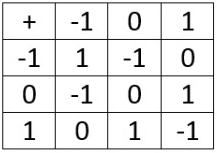
\includegraphics[scale=0.6]{tabela.png}
                    \caption{Tabela de Cayley de GF($3$)}
                    \label{Rotulo}
                \end{figure}
            
                
            \section{Curvas Elípticas}
                \tab Algumas propriedades das curvas elípticas, como sua forma, já foram discutidas nos tópicos anteriores, entretanto, existem outras características interessantes, que servem de motivação para o desenvolvimento das fórmulas para a criptografia de curvas elípticas.
                
                \begin{enumerate}
                    \item Como os pontos de uma curva elíptica formam uma estrutura de grupo, pode-se definir a ``soma'' entre seus pontos. Como visto anteriormente, tem-se um ponto chamado de ponto no infinito ${\Im}$, que é o elemento neutro da soma. Assim, seja $\Omega$ uma curva elíptica sobre um corpo $\mathbb{F} = \left\{ 0,1,2,...\right\}$ (assume-se que $\mathbb{F}$ é um corpo de característica\footnote{Característica é ``módulo'', ou seja, $\mathbb{F}_{a}$ seria o conjunto dos números de $0$ a $a-1$} maior que 3) e $P\in \Omega$ , tem-se:
                        
                    $$R \oplus {\Im} = {\Im} \oplus R= R$$
                    
                    o simétrico de um ponto $R= (x_R, y_R)$ é o ponto $-R = (x_R, -y_R)$, ou seja, naturalmente, tem-se:
                    $$R \oplus (-R) = {\Im} = (-R) \oplus R$$

                    \item Sejam $R$ e $Q$ dois pontos de uma curva elíptica sobre o corpo $\mathbb{R}$ dos números reais, tome a reta formada pelo segmento $\overline{PQ}$, esta reta intercepta a curva em um ponto $-R$. O simétrico de $-R$, que é dado por $R$, será a soma de $P$ e $Q$. Logo:
                        
                    $$R = P \oplus Q$$
                        
                    Dessa forma, é possível apelar para uma visualização geométrica para facilitar o entendimento, note que na representação geométrica, toma-se a curva elíptica como uma curva definida no $\mathbb{R}^2$, para que a continuidade natural da curva ajudasse no entendimento.
                        \\
                        \\
                        \\
                        \\
                        \\
                        \\
                        \\
                    \begin{figure}
                        \centering
                        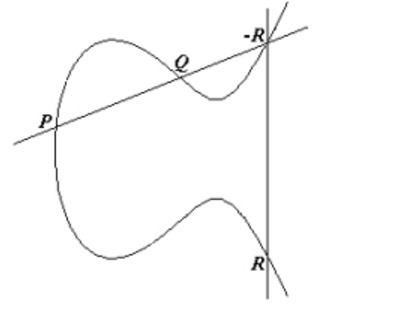
\includegraphics[scale=0.5]{geometrico.jpeg}
                        \caption{Representação Geométrica da Soma}
                        \label{fig:my_label}
                        \end{figure}
                    \end{enumerate}
                    
        \chapter{Teoria dos Números}
            \tab Como o projeto tomou como base curvas elípticas numa situação de aritmética módulo $p$, é necessário entender bem o conceito por trás de tal aritmética, e, na matemática, o ramo de estudo que foca nos números inteiros se chama Teoria dos Números, por isso, é bastante importante dominar a teoria para que o entendimento do projeto seja pleno.
                
            \section{Divisibilidade}
                \begin{defn}Dados os inteiros $a$ e $b$, não nulos, diz-se que $a$ é divisível por $b$ (escreve-se $b\mid a$), se existe um inteiro $k$, tal que $a = kb$. Alternativamente, $b\mid a$ pode ser lido como \textit{b é um divisor de a}, \textit{b é um fator de a} ou \textit{a é um múltiplo de b}.
                \end{defn}
                \tab Ainda, para quaisquer $a$,$b$ e $c$ inteiros, tem-se:
                \begin{itemize}
                    \item Se $a\mid b$ e $b\mid c$, então $a\mid (bx + cy)$, onde $bx + cy$ representa uma combinação linear de $b$ e $c$.
                \end{itemize}
                    
            \section{Máximo Divisor Comum}
                \begin{defn}Dados os inteiros $a$ e $b$, com pelo menos um deles diferente de zero, o inteiro positivo $d$ é dito ser o Máximo Divisor Comum entre $a$ e $b$, denotado por mdc$(a,b)$, se:
                \begin{enumerate}[label=(\roman*)]
                    \item $d\mid a$ e $d\mid b$.
                    \item Se $c\mid a$ e $c\mid b$, então $c\mid d$.
                \end{enumerate}
                \end{defn}
                \tab Ainda, se $d = \textrm{mdc}(a,b)$ então existem inteiros $x$ e $y$ tais que: $d = ax + by$, ou seja, o mdc entre dois inteiros $a$ e $b$ pode ser expresso como uma combinação linear dos mesmos.
                    
            \section{Números Primos}
                \begin{defn}O inteiro $p > 1$ é dito ser um número primo se não existe nenhum divisor de $p$ satisfazendo $1 < d < p$. Ou seja, são os números naturais que tem apenas dois divisores: o $1$ e ele mesmo. Se $n > 1$ não é primo, $n$ é dito ser um número composto.
                \end{defn}
                \tab Existem infinitos números primos, como demonstrado por Euclides por volta de $300$ a.C.. O conceito de número primo é muito importante na Teoria dos Números. Um dos resultados da Teoria dos Números é o \textbf{Teorema Fundamental da Aritmética}, que afirma que qualquer número natural diferente de $1$ pode ser escrito de forma única (desconsiderando a ordem) como um produto de números primos: este processo se chama decomposição em fatores primos (fatoração).
                    
            \section{Aritmética Modular}
                \tab Uma das ferramentas mais importantes na Teoria dos Números é a aritmética modular, que é um sistema de aritmética para inteiros, onde os números ``voltam pra trás'' quando atingem um certo valor, o módulo. Essa ferramenta envolve o conceito de congruência que será apresentado a seguir.
                    
                \subsection{Congruências Lineares}
                    \tab É um conceito muito importante e que está relacionado com divisibilidade e os restos de uma divisão de números inteiros. Uma congruência é a relação entre dois números que, divididos por um terceiro - chamado módulo de congruência - deixam o mesmo resto. Por exemplo, o número $10$ é congruente ao número $3$, módulo $7$, pois ambos deixam resto $3$, ao serem divididos por $7$.
                    \begin{defn}Em suma, para um inteiro positivo $n$, dois inteiros $a$ e $b$ são ditos congruentes módulo $n$, e escreve-se: $a\equiv b \textrm{ }(\textrm{mod } n)$ quando a diferença deles $a - b$ é um inteiro múltiplo de $n$. O número $n$ é chamado o módulo da congruência.
                    \end{defn}
                    \tab Algumas propriedades das congruências lineares são apresentadas a seguir:
                    \begin{enumerate}[label=(\roman*)]
                        \item Se $a\equiv b \textrm{ }(\textrm{mod } n)$ e $b\equiv c \textrm{ }(\textrm{mod } n)$, então $a\equiv c \textrm{ }(\textrm{mod } n)$.
                        \item Se $a\equiv b \textrm{ }(\textrm{mod } n)$ e $d \mid n$, $d>0$, então $a\equiv b \textrm{ }(\textrm{mod } d)$
                        \item Se $ca\equiv cb \textrm{ }(\textrm{mod } n)$, então $a\equiv b \textrm{ }(\textrm{mod } \frac{n}{d})$, em que $d = \textrm{mdc }(c,n)$.
                        \item $a\equiv b \textrm{ }(\textrm{mod } pq)$ se e só se $a\equiv b \textrm{ }(\textrm{mod } p)$ e $a\equiv b \textrm{ }(\textrm{mod } q)$, em que $p$ e $q$ são primos distintos.
                    \end{enumerate}
                
                \subsection{Teste de Miller-Rabin}
                    \tab  O teste de Miller-Rabin é um teste probabilístico da primalidade de um dado número $n$. Se um número $n$ não passar pelo teste, $n$ com certeza é um número composto. Se o número passar no teste, ele é primo, com uma probabilidade $P(n\in G) \geq 0.75$, sendo que $G$, nesse caso, denomina o conjunto de todos números primos. \\
                    \tab É importante dizer que o teste de Miller-Rabin não dá indícios sobre a fatoração no número $n$. Devido a suas características, esse teste é o mais utilizado para o teste de primalidade, embora, à risca, este seja um teste de compositividade. \\
                    \tab O teste afirma que, seja $n$ um número primo e $a$ um número inteiro escolhido aleatoriamente, tal que $1 < a < p$. Seja $s = \textrm{max } \left\{r\in \N : 2^r \textrm{ divide } (n-1)\right\}$. $s$ é o maior expoente, tal que $2^s\mid (n-1)$. Seja $d = (n-1) / 2^s$, por definição de $s$, $d$ é, necessariamente, ímpar.
                    \begin{teorema} Se $n$ é um número primo e $a$ não tiver um divisor em comum com $p$, então $$a^d\equiv 1\textrm{ }(\textrm{mod } n) \textrm{ ou existe um }r\in \left\{0,1,...,s-1\right\}\textrm{, tal que } a^{2^rd}\equiv -1 \textrm{ }(\text{mod } n)$$
                    \end{teorema}
                    Um número $a$ que não satisfaz o teorema acima é denominado de testemunha contra a primalidade de $n$.
            
        \chapter{Implementação}
            \tab Para iniciar a implementação da criptografia em curvas elípticas, foi necessário se apoiar em uma definição de soma de pontos da curva.
            \begin{defn}
            A soma de dois pontos, $P = (x_P , y_P )\textrm{ e } Q = (x_Q , y_Q )$, de uma CE, realizada através da operação binária denotada por $\oplus$, é definida como $R = (x_R , y_R )$, em que
            \begin{itemize}
                \item Se $x_P \equiv x_Q\textrm{ }(\textrm{mod }p)$ e $y_P \equiv -y_Q\textrm{ }(\textrm{mod }p)$, então $R \equiv \Im\textrm{ }(\textrm{mod }p)$;
                \item Senão, $x_R \equiv t^2 - x_P - x_Q\textrm{ }(\textrm{mod }p) $, $y_R \equiv t(x_P - x_R ) - y_P\textrm{ }(\textrm{mod }p)$, em que
                    $$t \equiv 
                    \begin{cases} 
                    (y_Q-y_P)(x_Q-x_P)^{-1}\textrm{ }(\textrm{mod }p),\textrm{ se }P\neq Q \\
                    (3x_P^2+a)(2y_P)^{-1}\textrm{ }(\textrm{mod }p),\textrm{ se }P=Q
                    \end{cases}$$
                    
                \item Para todo $P$ pertencente à curva elíptica,
                $$P \oplus \Im = \Im \oplus P = P$$
            \end{itemize}
            \end{defn}
            
            \section{<CE, $\oplus$> é um grupo?}
                \begin{proof} 
                    Para determinar se <CE, $\oplus$> é, de fato, um grupo, deve-se recorrer à Definição 1, ou seja, deve-se checar se <CE, $\oplus$> é um conjunto de elementos que atende \textbf{Associatividade}, \textbf{Identidade}, \textbf{Inverso} e \textbf{Fechamento}.
                
                \subsection{Identidade}
                    \begin{proof} 
                        A existência e unicidade do elemento identidade decorre da própria Definição 7, no terceiro item, sendo a identidade de <CE, $\oplus$>, o ponto infinito $\Im$. 
                    \end{proof}
                \subsection{Inverso}
                    \begin{proof} 
                        A existência e unicidade do elemento inverso decorre da própria Definição 7, no primeiro item, sendo o inverso de $P = (x_P, y_P)$, o ponto $Q=(x_Q,y_Q)$, ou seja:
                        $$P \oplus Q = Q \oplus P = \Im$$.
                    \end{proof}
                    
                \subsection{Associatividade}
                    \begin{proof}
                        Seja $P=(x_P,y_P)$ e $Q = (x_Q, y_Q)$, é necessário separar a demonstração em 3 casos:
                        \begin{enumerate}
                            \item Se $P=Q$, então $x_P \equiv  x_Q\textrm{ }(\textrm{mod }p)$ e $y_P \equiv y_Q\textrm{ }(\textrm{mod }p)$, logo:
                                \begin{enumerate}
                                    \item $P\oplus Q$ \\
                                    $$x_{P+Q} \equiv \left(\frac{3x_P^2 + a}{2y_P}\right)^2 -2x_P\textrm{ }(\textrm{mod }p)$$
                                    $$y_{P+Q} \equiv \left(\frac{3x_P^2 + a}{2y_P}\right)^2(x_P-x_{P+Q}) - y_P\textrm{ }(\textrm{mod }p)$$
                                    
                                    \item $Q\oplus P$ \\
                                    $$x_{Q+P} \equiv \left(\frac{3x_P^2 + a}{2y_P}\right)^2 -2x_P\textrm{ }(\textrm{mod }p) \equiv x_{P+Q}\textrm{ }(\textrm{mod }p)$$
                                    $$y_{Q+P} \equiv \left(\frac{3x_P^2 + a}{2y_P}\right)^2(x_P-x_{Q+P}) - y_P\textrm{ }(\textrm{mod }p) \equiv \left(\frac{3x_P^2 + a}{2y_P}\right)^2(x_P-x_{P+Q}) - y_P\textrm{ }(\textrm{mod }p) \equiv y_{P+Q}\textrm{ }(\textrm{mod }p)$$
                                    
                                    Logo, $x_{P+Q} \equiv x_{Q+P}\textrm{ }(\textrm{mod }p)$ e $y_{P+Q} \equiv y_{Q+P}\textrm{ }(\textrm{mod }p)$, então 
                                    $$P \oplus Q = Q \oplus P$$
                                \end{enumerate}
                            \item Se $P = (x_P,y_P)$ e $Q = (x_P, -y_P)$, tem-se que $P$ é o inverso de $Q$, logo
                                $$P\oplus Q = Q\oplus P = \Im$$
                            \item Senão, seja $P = (x_P, y_P)$ e $Q = (x_Q,y_Q)$
                                \begin{enumerate}
                                    \item Se $P\oplus Q = R$, com $R = (x_R,y_R)$ \\
                                    \begin{equation}
                                    x_R = \left(\frac{y_Q - y_P}{x_Q - x_P}\right)^2 - x_P - x_Q\textrm{ }(\textrm{mod }p)    
                                    \end{equation}
                                    $$y_R = \left(\frac{y_Q - y_P}{x_Q - x_P}\right)(x_P - x_R) - y_P\textrm{ }(\textrm{mod }p)$$
                                    $$y_R = \left(\frac{y_Q - y_P}{x_Q - x_P}\right)(x_P - x_R) - y_P\frac{x_Q-x_P}{x_Q-x_P}\textrm{ }(\textrm{mod }p)$$
                                    \begin{equation}
                                    y_R = \frac{y_Px_Q -y_Px_R -y_Qx_Q+y_Qx_R -y_Qx_P + y_Qx_Q}{x_P - x_Q}\textrm{ }(\textrm{mod }p)
                                    \end{equation}
                                    \item Se $Q\oplus P = S$, com $S=(x_S, y_S)$
                                        $$x_S = \left(\frac{y_P - y_Q}{x_P - x_Q}\right)^2 - x_Q - x_P\textrm{ }(\textrm{mod }p)$$
                                        $$x_S=\left(\frac{y_Q - y_P}{x_Q - x_P}\right)^2 - x_Q - x_P\textrm{ }(\textrm{mod }p)$$
                                        \begin{equation}
                                            x_S=\left(\frac{y_Q - y_P}{x_Q - x_P}\right)^2 - x_P - x_Q\textrm{ }(\textrm{mod }p)
                                        \end{equation}
                                        Comparando $(4.3)$ com $(4.1)$, segue que: $
                                        $x_S=x_R$$
                                        
                                        $$ y_S = \left(\frac{y_P - y_Q}{x_P - x_Q}\right)(x_Q - x_S) - y_Q\textrm{ }(\textrm{mod }p)$$
                                        $$y_S = \left(\frac{y_P - y_Q}{x_P - x_Q}\right)(x_Q - x_S) - y_Q\frac{x_P-x_Q}{x_P-x_Q}\textrm{ }(\textrm{mod }p)$$
                                        \begin{equation}
                                            y_S = \frac{y_Px_Q -y_Px_S -y_Qx_Q+y_Qx_S -y_Qx_P + y_Qx_Q}{x_P - x_Q}\textrm{ }(\textrm{mod }p)
                                        \end{equation}
                                        Usando que $x_S=x_R$ e comparando $(4.4)$ com $(4.2)$: segue que 
                                        $$y_S=y_R$$ 
                                        Logo
                                        $$P \oplus Q = Q\oplus P$$
                                        
                                \end{enumerate}
                        \end{enumerate}
                        Nesses 3 casos, foi provado que vale a comutatividade para o conjunto <CE, $\oplus$>, mas se vale a comutatividade, vale a associatividade.
                    \end{proof}
                \subsection{Fechamento}
                    \begin{proof}
                        Para demonstrar o fechamento, é necessário analisar 3 casos:
                    
                        \begin{enumerate}
                            \item Sendo $P$ um ponto pertencente à curva elíptica
                            $$P \oplus \Im = P$$
                            Logo, segue trivialmente que a operação com a identidade é fechada.
                            \item Sendo $P$ um ponto pertencente à curva elíptica
                            $$P \oplus P^{-1} = \Im$$
                            Como $\Im$ é o elemento identidade da curva elíptica, segue que um elemento operado com seu inverso é fechado.
                            \item Toma-se $P = (x_P, y_P)$, $Q = (x_Q, y_Q)$ e $R = (x_R, y_R)$, tal que $P \oplus Q = R$, onde $P$ e $Q$ são pontos da curva elíptica.\\ \\
                            Para provar que $R$ também é um ponto da curva elíptica, pode-se usar a inspiração geométrica mencionada anteriormente. \\ \\
                            Usando a ideia de reta, pode-se escrever que:
                            \begin{equation}
                                y \equiv y_P + t(x-x_P) \textrm{ }(\textrm{mod }p)
                            \end{equation}
                            Onde $t \equiv \begin{cases}
                            (y_P - y_Q)(x_P - x_Q)^{-1} \textrm{ }(\textrm{mod }p),\textrm{ se }P=Q\\
                            (3x_P^2+a)(2y_Q)^{-1} \textrm{ }(\textrm{mod }p),\textrm{ se }P\neq Q
                            \end{cases}$ \\ \\ \\
                            Substituindo $y$ na Equação $(1.1)$ para a curva elíptica:
                            $$(y_P + t(x-x_P))^2 \equiv x^3 +ax + b \textrm{ }(\textrm{mod }p)$$
                            $$y_P^2 + 2ty_P(x-x_P) + t^2(x-x_P)^2 \equiv x^3 +ax + b \textrm{ }(\textrm{mod }p)$$
                            $$x^3 +ax + b - y_P^2 -2ty_Px + 2ty_Px_P-t^2x^2+2t^2xx_P-t^2x_P^2 \equiv 0 \textrm{ }(\textrm{mod }p)$$
                        
                            Já que na curva elíptica não é possível ter raízes múltiplas, por conta da Equação $(1.2)$ a equação acima possui $3$ soluções distintas em módulo $p$. Como duas dessas soluções são conhecidas, $x_P$ e $x_Q$, a outra solução só pode ser $x_S = x_R$. Sendo assim, pela expressão de Vieta\footnote{Alguns chamam essa expressão de uma das Relações de Girard} da soma, temos:
                            $$\frac{-t^2}{-1} \equiv x_P + x_Q + x_S\textrm{ }(\textrm{mod }p)$$
                            \begin{equation}
                                x_S \equiv t^2 - x_P - x_Q\textrm{ }(\textrm{mod }p)
                            \end{equation}
                            Usando $(4.2)$ em $(4.1)$:
                            $$y_S \equiv y_P + t(x_S - x_P)\textrm{ }(\textrm{mod }p)$$
                            Para finalizar, inverte-se o sinal do ponto $S = (x_S, y_S)$, visto que a solução $R=(x_R,y_R)$ é o inverso de $S$, ou seja, $R = (x_S, -y_S)$:
                            $$y_R = -y_S = t(x_P-x_R) - y_P\textrm{ }(\textrm{mod }p)$$
                            Que é uma equação de reta que tem ``coeficiente angular'' de mesmo valor absoluto que o de $y_S$, sendo que com sinal inverso, assim como seu ``coeficiente linear''. 
                        \end{enumerate}
                    \end{proof}
                    Como as 4 condições foram atendidas, <CE, $\oplus$> é sim um grupo, e mais que isso, <CE, $\oplus$> é um grupo abeliano.
                \end{proof}
                
            \section{Algorítmo para $\oplus$}
                \tab Para realizar a implementação do algorítmo que realiza a operação $\oplus$, foi usado a linguagem de programação \textit{Python 3} principalmente por conta do tamanho de \textit{bits} que a variável genérica \textit{int} suporta, que supera (e muito) o necessário ($512\textit{ }bits$). Segue abaixo o código implementado
                
                \inputpython{scalarecc.py}{7}{19}
                \inputpython{scalarecc.py}{20}{26}
                \inputpython{scalarecc.py}{5}{6}
                
                \tab Onde a função \pyth{ecadd()} representa a operação $\oplus$ para dois pontos distintos, e a função \pyth{ecdbl()} representa a operação $\oplus$ para dois pontos iguais. Para auxiliar na implementação, foi usado a função \pyth{modinv()} que basicamente retorna o inverso multiplicativo para um dado resíduo.
                

            \section{Algorítmo para $P^N$}
                \tab Segue abaixo a implementação do algorítmo que realiza a operação $P^N=\underbrace{P\oplus P\oplus \ldots \oplus  P}_{N\text{vezes}}$
                
                \inputpython{scalarecc.py}{27}{34}
                
                Nota-se, pelo código, que sempre que um dígito da representação binária do número $N$ for $1$, o algorítmo irá fazer a operação \pyth{ecadd()}. A quantidade de $1$ na representação binária do número $N$ nada mais é que o seu peso de Hamming, logo, tem-se que o número máximo de adições necessárias em função da quantidade de \textit{bits} de $N$ será o peso de Hamming da representação em binário de $N$
                
            \section{Segurança de <CE, $\oplus$>}
                \subsection{Ordem de <CE, $\oplus$>}
                    \tab Por motivos a serem clarificados na seção da implementação do protocolo de ElGamal, foi escolhido um primo $p$ da forma $p=4k+3$. Isso implica que para cada $x \in \mathbb{F}_p$ tem-se $2$ valores possíveis para $y$. Como $x$ varia de $0$ a $p-1$, tem-se então que o conjunto dos pontos da curva elíptica possui $2p$ elementos, e portanto sua ordem é $2p$.
                    
                \subsection{Logarítmo Discreto}
                    \tab O problema de resolver logarítmos discretos é bem famoso na história da computação, e trata-se, de, sabendo os valores $b$ e $a$, encontrar o valor $N$ tal que
                    $$a^N = b$$
                    \tab Esse problema é dito díficil de resolver pois, assim como na fatoração de números inteiros, não existe, até os dias de hoje, um algorítmo eficiente\footnote{Neste artigo, considera-se um algorítmo eficiente aquele que resolve o problema em tempo polinomial}  que calcule o logarítmo discreto. \\
                    \tab Por conta da ineficiência desses algorítmos, sistemas criptográficos modernos, como a criptografia em curvas elípticas, surgiram com bastante presença, visto que é inviável encontrar um resultado de logaritmo através do uso de força bruta. Portanto, assume-se que o indivíduo que queira quebrar o sistema criptográfico nunca conseguirá faze-lo caso não tenha acesso a alguma informação privada.
                    
            \section{ElGamal sobre Curvas Elípticas}
                \tab O protocolo de ElGamal é uma forma de dois indivíduos $A$ e $B$ trocarem mensagens por um canal inseguro sem que a mensagem seja alterada e que se tenha a garantia da autenticação da assinatura da mensagem. O algoritmo funciona da seguinte forma:
                \begin{itemize}
                    \item \textbf{Inicialização:} O sistema gera os parâmetros públicos, no caso do ElGamal, o elemento $P$ gerador e um $p$ que seria um primo tomado como resíduo que define a aritmética tal qual o algoritmo funcionará
                    \item \textbf{Autenticação:} O indivíduo $A$ envia para o indivíduo $B$ o gerador $P$ elevado à potência de sua chave privada $x$, chama-se $P^x = H$
                    \item \textbf{Criptografia:} O indivíduo $B$, em posse de $H$, eleva este à sua chave privada $y$, dessa forma, obtendo $S = H^y = P^{xy}$, chamado segredo compartilhado. Em posse de $S$, $B$ irá calcular $2$ valores: $C_1$ e $C_2$, sendo $C_1 = P^y$, e $C_2 = M\oplus S$, onde $M$ é o mapeamento bijetivo entre a mensagem que $B$ pretende enviar e um ponto na curva elíptica e $C_1$ é a assinatura da troca de mensagens já que $A$ poderá verificar se $B$ realmente enviou a mensagem vendo se $C_1$ fornece o $S$ correto para descriptografar a mensagem.
                    \item \textbf{Descriptografia:} $A$ irá receber $C_1$ e $C_2$ e irá calcular o $M$ fazendo, primeiramente $S = C_1^x$, em posse de $S$, $A$ irá calcular o inverso de $S$, chamado $S^{-1}$, e então fará $$C_2\oplus S^{-1} = M\oplus H^y \oplus S^{-1} = M\oplus S \oplus S^{-1} = M$$
                \end{itemize}
                \tab Para implementação da criptografia sob curvas elípticas, foi utilizado o protocolo de ElGamal. Um grande desafio nessa implementação foi como mapear uma mensagem para um ponto único sob a curva, disso, entra a justificativa de usar um $p=4k+3$. Sabe-se que um ponto\footnote{Ao longo desta seção é conveniente utilizar o abuso de notação de não se preocupar com o módulo $p$, visto que $p$ foi considerado tão grande quanto o necessário para mapear qualquer mensagem unicamente} da curva elíptica $P$ é tal que $P=(x,\sqrt{x^3 + ax + b})$, onde $x$ é um número associado à mensagem, como para um dado $x$, deve-se calcular um $y$ relacionado, uma condição possível para que haja exatamente $2$ resultados para $x$, é que o primo $p$ seja da forma $p = 4k+3$, já que é necessário que se tenha apenas um valor para $y$, foi arbitrariamente escolhido que o valor de $y$ será o resultado positivo da solução da equação quadrática.
                
                \tab Abaixo, segue a implementação em \textit{Python 3} da criptografia elíptica com protocolo de ElGamal
                \inputpython{discretos.py}{118}{146}
                \inputpython{discretos.py}{147}{153}
                \inputpython{discretos.py}{2}{87}
                \\
                \tab Onde a primeira caixa de código representa as funções principais do ElGamal, enquanto as duas outras caixas de código representam funções auxiliares que ajudaram na implementação.
                
        
        \chapter{Análise}
            Nesta seção serão discutidos possíveis ataques ao sistema criptográfico utilizando o protocolo de ElGamal implementado sobre curvas elípticas.
            \section{Ataque do Homem do Meio}
                Neste ataque, é suposto uma situação em que dois indivíduos, \textit{Alice} e \textit{Bob}, trocam mensagens usando o protocolo de ElGamal por um canal inseguro. Durante uma troca de mensagens, um terceiro malicioso intercepta um envio, e, sabendo, por outros meios, o que a mensagem representa e como está criptografada, é possível quebrar o sistema da seguinte maneira:
                \begin{itemize}
                    \item \textit{Charlie}, o terceiro malicioso, recebe a mensagem criptografada $C_2$ e o que ela realmente significa $M$ 
                    \item Sabendo que $C_2 \oplus S^{-1} = M$, \textit{Charlie} pode operar $C_2^{-1}$ dos dois lados, visto que é facil descobrir inversos em curvas elípticas, e com isso Charlie descobre $S^{-1} = C_2^{-1}\oplus M$
                    \item Sabendo $S^{-1}$, novamente, é muito fácil obter o inverso, então agora \textit{Charlie} possui $S$
                    \item Em posse de $S$, \textit{Charlie} pode agora descriptografar qualquer mensagem trocada, visto que para descobrir uma mensagem, basta operar $S^{-1}$ com as mensagens
                \end{itemize}
                
            \section{Força Bruta}
                É o ataque trivial. Neste ataque testa-se todos os valores possíveis para $i$ na equação 
                $$P^i = H$$
                Para buscar o $i = x$. Note que nesse caso o sujeito que ataca tem que interceptar alguma mensagem, mas diferente do homem do meio, o sujeito não sabe o que aquela mensagem interceptada significa realmente.
                
            \section{Casos Particulares de Ordem}
                Se a ordem do grupo das curvas elípticas for um primo $p$, um número do tipo $p+1$ ou $p-1$, ou até um produto entre primos pequenos, existem alguns algorítmos conhecidos para atacar o problema do logarítmo discreto, mas a demonstração desses algorítmos está fora do escopo desse trabalho.
        \chapter{Conclusão}
            \tab Após a implementação da criptografia em curvas elípticas, foi possível observar que a mensagem é recebida com segurança caso a ordem não seja um número primo, um número do tipo $p+1$ ou $p-1$, e que também não seja um número tal que possa ser fatorado em dois primos razoavelmente pequenos, além de que, o algoritmo de criptografia em curvas elípticas usando o protocolo de ElGamal assegura a autenticidade do envio/recebimento da mensagem. \\
            \tab Um fato muito interessante que também foi observado é que o tamanho da chave privada usada é muito menor do que as implementações do protocolo de ElGamal que não usam curvas elípticas. Graças a essa portabilidade, evidencia-se o possível uso da criptografia de curvas elípticas em aplicações onde a memória é limitada, tais como sistemas baseados em IoT (Internet of Things), ou em aplicações que necessitam um alto grau de segurança, a exemplo do \textit{bitcoin}.
            
            \begin{thebibliography}{1}

                \bibitem{impj} RYKWALDER, {\em Eric. The Math Behind Bitcoin}. 2014. Disponível em: <https://www.coindesk.com/math-behind-bitcoin/>. Acesso em: 08 dez. 2017.

                \bibitem{impj}  KARTHIKEYAN, E. {\em Survey of Elliptic Curve Scalar Multiplication Algorithms.} [23/08/2012]. 10 p. Artigo (Computer Science)- Government Arts College, India, 2012. Disponível em: <http://www.ijana.in/papers/V4I2-8.pdf>. Acesso em: 10 dez. 2017. 

                \bibitem{norman} PRIESTLEY, H. A. . {\em Introduction to Groups, Rings and Fields.} 2011. 45 f. Groups,FIelds and RIngs (Introduction to Groups, Rings and Fields, Maths) [S.l.], 2011.

                \bibitem{impj} LARA, Pedro Carlos da Silva; DE OLIVEIRA, Fábio Borges. {\em Curvas Elípticas: Aplicação em Criptografia Assimétrica.} 10 p. Artigo (Ciência da Computação)- Laboratório Nacional de Computação Científica – LNCC, Petrópolis. RJ. Acesso em: 08 dez. 2017. 

                \bibitem{impj} AN, Junfeng et al. {\em State-of-the-art of secure ECC implementations: a survey on known side-channel attacks and countermeasures.} 2010. 12 f. - Katholieke Universiteit Leuven, [S.l.], 2010.
                
                \bibitem{impj} CAMPELLO, Ricardo. {\em Apostila de Sistema Discretos}. Recife: UFPE. 80 p.
                
                \bibitem{impj} STEIN, WIlliam. {\em The Elliptic Curve Discrete Logarithm Problem}. Disponível em: <http://wstein.org/edu/2007/spring/ent/ent-html/node89.html>. Acesso em: 12 dez. 2017.
                
                \bibitem{impj} CORBELLINI, Andrea. {\em Elliptic Curve Cryptography: breaking security and a comparison with RSA}. Disponível em: <http://andrea.corbellini.name/2015/06/08/elliptic-curve-cryptography-breaking-security-and-a-comparison-with-rsa/>. Acesso em: 12 dez. 2017.
            \end{thebibliography}
\end{document}